\documentclass[oneside]{report}
\usepackage{hyperref}
\usepackage{url}
\usepackage{graphicx}
\usepackage{listings}
\usepackage{float}  
\usepackage{color, colortbl}
\usepackage{svg}
\usepackage{xepersian}
\setcounter{tocdepth}{4}
\setcounter{secnumdepth}{4}
\renewcommand{\thesection}{\arabic{section}}
\hypersetup{colorlinks=true , allcolors=blue}
\settextfont{XB Niloofar}
\title{
      بسم اللّه الرحمن الرحیم
      \\[2cm]
    
\includegraphics[width=0.5\linewidth]{../images/iust.png}
    \\
    پروژه Samarium درس شبکه های تلفن همراه
    }
    \author{محمد صادق پولائی موزیرجی - 99521145 \\ 
    \and سبحان کاظمی - 99522023}
    \date{تابستان 1403}

    \definecolor{excellent_color}{HTML}{00703C}
    \definecolor{very_good_color}{HTML}{00A032}
    \definecolor{good_color}{HTML}{00D228}

    \definecolor{fair_color}{HTML}{FFFF00}
    \definecolor{poor_color}{HTML}{FFAA00}
    \definecolor{very_poor_color}{HTML}{FA6400}
    \definecolor{bad_color}{HTML}{FF0000}
    \definecolor{very_bad_color}{HTML}{DC133C}
    \definecolor{awful_color}{HTML}{820000}
    \definecolor{no_coverage_color}{HTML}{AAAAAA}
    
\begin{document}

\maketitle
\tableofcontents
\listoffigures
\baselineskip = 0.85cm
\newpage

\section{مقدمه}
ساماریوم یک برنامه شبکه‌ای جانبی است که برای دستگاه‌های اندروید توسعه داده شده است و به کاربران امکان می‌دهد کیفیت خدمات (QoS) را در شبکه‌های سلولی هنگام حرکت اندازه‌گیری کنند. این برنامه موقعیت مکانی زنده کاربر را با استفاده از API های خدمات موقعیت مکانی گوگل پلی ردیابی می‌کند و در عین حال اطلاعات سلول‌ها را با استفاده از API های مخابراتی اندروید استخراج می‌کند. علاوه بر این، این برنامه در مکان‌های غیرقابل دسترسی مانند تونل‌ها با استفاده از روش اقلیدسی به درستی عمل می‌کند. پارامترهای زیر برخی از شاخص‌های شبکه‌ای هستند که ساماریوم قادر به استخراج آنهاست:
\begin{itemize}
      \item پارامترهای شاخص کیفیت سیگنال در 4G و 3G مانند RSRQ، \lr{EC/N0}
      \item پارامترهای شاخص کمیت سیگنال در 4G و 3G مانند RSRP، RSCP
      \item اطلاعات خاص سلول مانند PLMN، LAC، TAC
\end{itemize}
اطلاعات بازیابی شده در پایان روی نقشه نمایش داده می‌شوند. جدول زیر نشان می‌دهد که چگونه اطلاعات روی نقشه نمایش داده می‌شوند:
\begin{table}[h!]
      \centering
      \begin{tabular}{|c|c|c|}
            \hline
            رنگ                           & بازه               & تفسیر سیگنال \\
            \hline
            \cellcolor{excellent_color}   & $-80 < x < \infty$ & عالی         \\
            \hline
            \cellcolor{very_good_color}   & $-85 < x < -80$    & بسیار خوب    \\
            \hline
            \cellcolor{good_color}        & $-90 < x < -85$    & خوب          \\
            \hline
            \cellcolor{fair_color}        & $-95 < x < -90$    & قابل قبول    \\
            \hline
            \cellcolor{poor_color}        & $-100 < x < -95$   & ضعیف         \\
            \hline
            \cellcolor{very_poor_color}   & $-105 < x < -100$  & بسیار ضعیف   \\
            \hline
            \cellcolor{bad_color}         & $-110 < x < -105$  & بد           \\
            \hline
            \cellcolor{very_bad_color}    & $-115 < x < -110$  & بسیار بد     \\
            \hline
            \cellcolor{awful_color}       & $-120 < x < -115$  & وحشتناک      \\
            \hline
            \cellcolor{no_coverage_color} & بدون پوشش          & تعریف نشده   \\
            \hline
      \end{tabular}
      \caption{نحوه نمایش اطلاعات سیگنال روی نقشه}
      \label{table:signal}
\end{table}

\section{ویژگی‌های پیشنهادی}
\subsection{اعتبارسنجی مجوز}
برنامه به مجوزهایی مانند دسترسی به موقعیت مکانی نیاز دارد تا بدون مشکل کار کند. بنابراین، در صورت عدم اعطای مجوزهای لازم، هنگام راه‌اندازی درخواست مجوز می‌کند.
\begin{itemize}
      \item مجوز دسترسی به موقعیت مکانی
      \item درخواست فعال‌سازی GPS
\end{itemize}
\begin{center}
      \begin{figure}[H]
            \centering
            
\includegraphics[width=0.4\textwidth]{../images/loc-perm.jpg}
            \caption{اعتبارسنجی مجوز دسترسی به موقعیت مکانی}
      \end{figure}
      \begin{figure}[H]
            \centering
            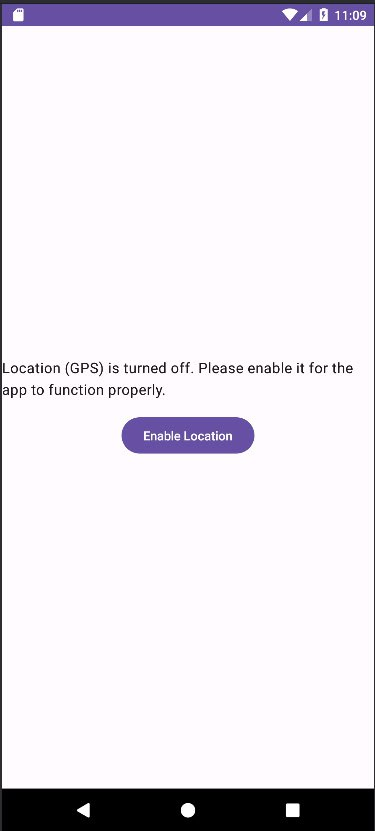
\includegraphics[width=0.4\textwidth]{../images/gps-enable.jpg}
            \caption{درخواست فعال‌سازی GPS}
      \end{figure}
\end{center}
\textbf{اگرچه مجوز دسترسی به موقعیت مکانی لازم است، سرویس GPS نیز باید فعال باشد تا برنامه بتواند به خوبی کار کند.}

\subsection{سفارشی‌سازی تنظیمات}
\begin{itemize}
      \item به طور کلی، برنامه هر 10 ثانیه یک بار اطلاعات را به‌روزرسانی می‌کند. با این حال، این تنظیمات می‌تواند از طریق پنل تنظیمات تغییر کند.
      \item پایگاه داده داخلی که حاوی اطلاعات برنامه است نیز می‌تواند برای افزایش سرعت پاکسازی شود.
\end{itemize}
\begin{center}
      \begin{figure}[H]
            \centering
            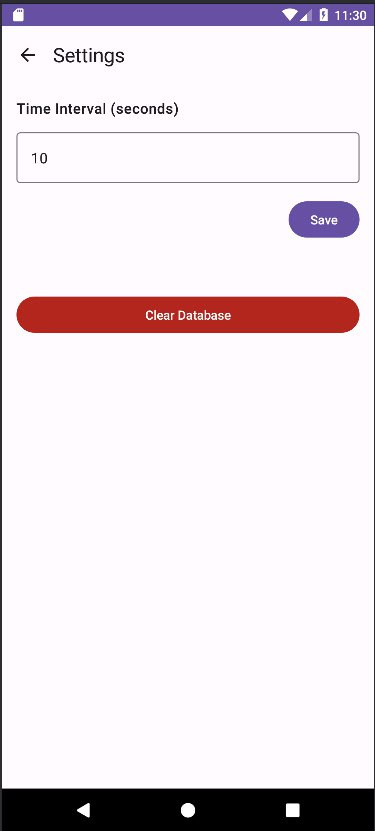
\includegraphics[width=0.4\textwidth]{../images/setting.jpg}
            \caption{پنل تنظیمات}
      \end{figure}
\end{center}

\subsection{برآورد موقعیت مکانی}
در مواقعی که GPS خدمات ارائه نمی‌دهد، دسترسی به موقعیت مکانی از طریق GPS ممکن است در دسترس نباشد و موقعیت فعلی کاربر باید به روشی تخمین زده شود. ساماریوم از روش اقلیدسی برای تخمین موقعیت دقیق کاربر استفاده می‌کند. به طور کلی، از آخرین موقعیت مکانی شناخته شده قبل از قطع اتصال GPS و اولین موقعیت مکانی در دسترس پس از اتصال مجدد GPS برای تقریبی طول و عرض جغرافیایی مکان‌های غیرقابل دسترس استفاده می‌کند. در نهایت، فاصله نامشخص را به بخش‌های مساوی تقسیم می‌کند تا طول و عرض جغرافیایی تقریبی را به آنها اختصاص دهد. عملکرد اصلی این روش در مسیر `/app/src/main/java/ir/tehranshomal/samarium/Services/InformationFetchService.kt` از ساختار برنامه پیاده‌سازی شده است.

\section{وضعیت زنده کاربر}
\begin{itemize}
      \item وضعیت فعلی کاربر گرفته شده و روی نقشه نمایش داده می‌شود. تصاویر زیر نقشه حرارتی کاربر را در خیابان‌های تهران نشان می‌دهند.
\end{itemize}
\begin{center}
      \begin{figure}[H]
            \centering
            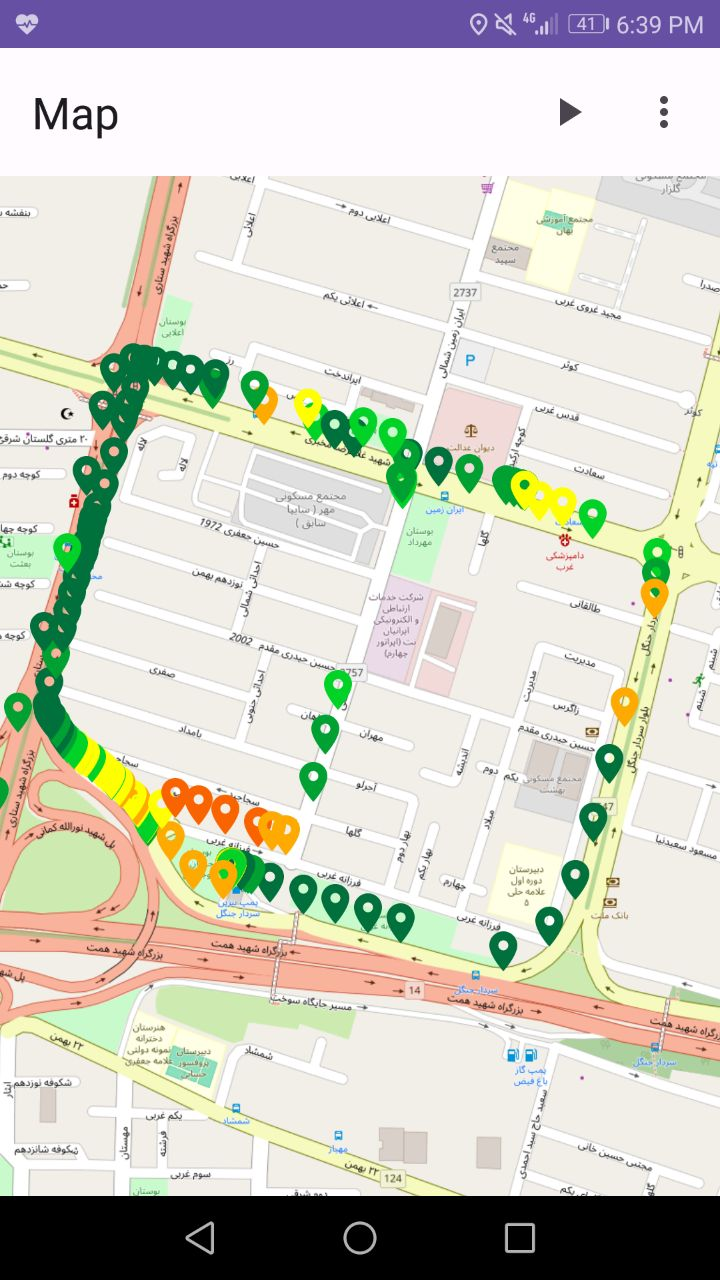
\includegraphics[width=0.4\textwidth]{../images/map1.jpg}
            \caption{نقشه حرارتی کاربر در خیابان‌های تهران}
      \end{figure}
      \begin{figure}[H]
            \centering
            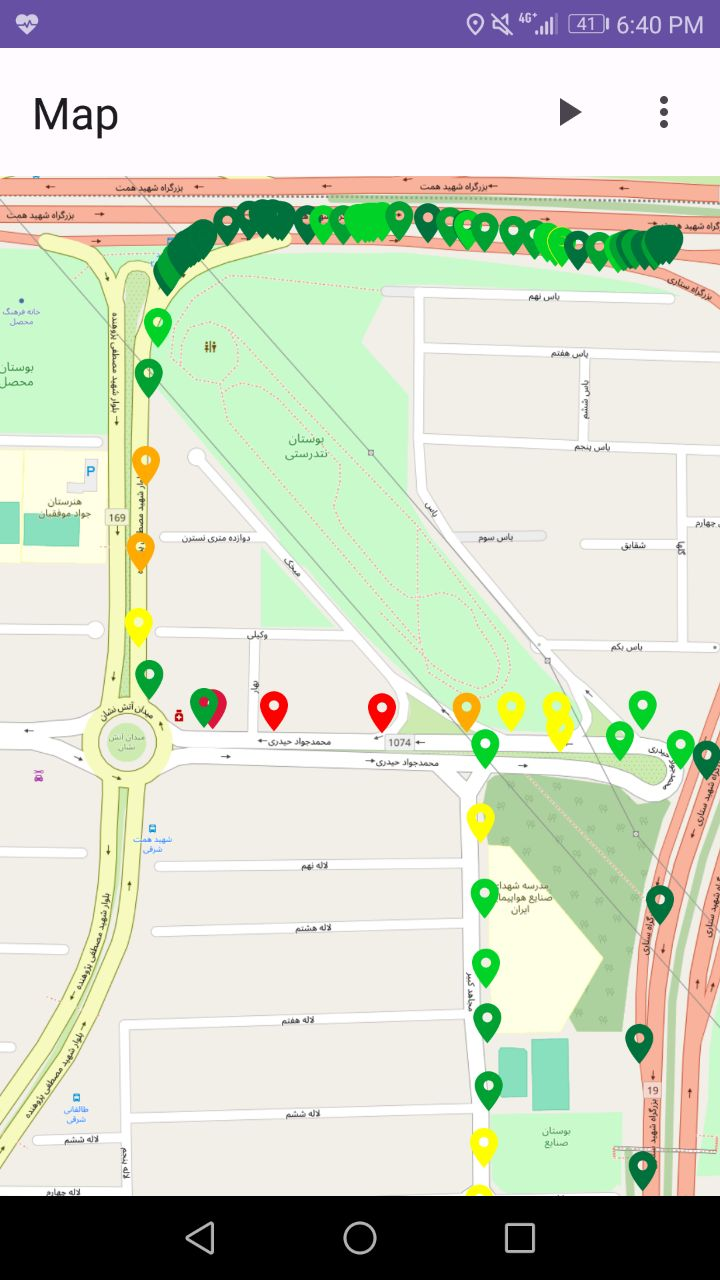
\includegraphics[width=0.4\textwidth]{../images/map2.jpg}
            \caption{نقشه حرارتی کاربر در خیابان‌های تهران -2}
      \end{figure}
\end{center}

\begin{itemize}
      \item اطلاعات مربوط به هر نقطه ثبت شده به صورت زیر نمایش داده می‌شود.
\end{itemize}
\begin{center}
      \begin{figure}[H]
            \centering
            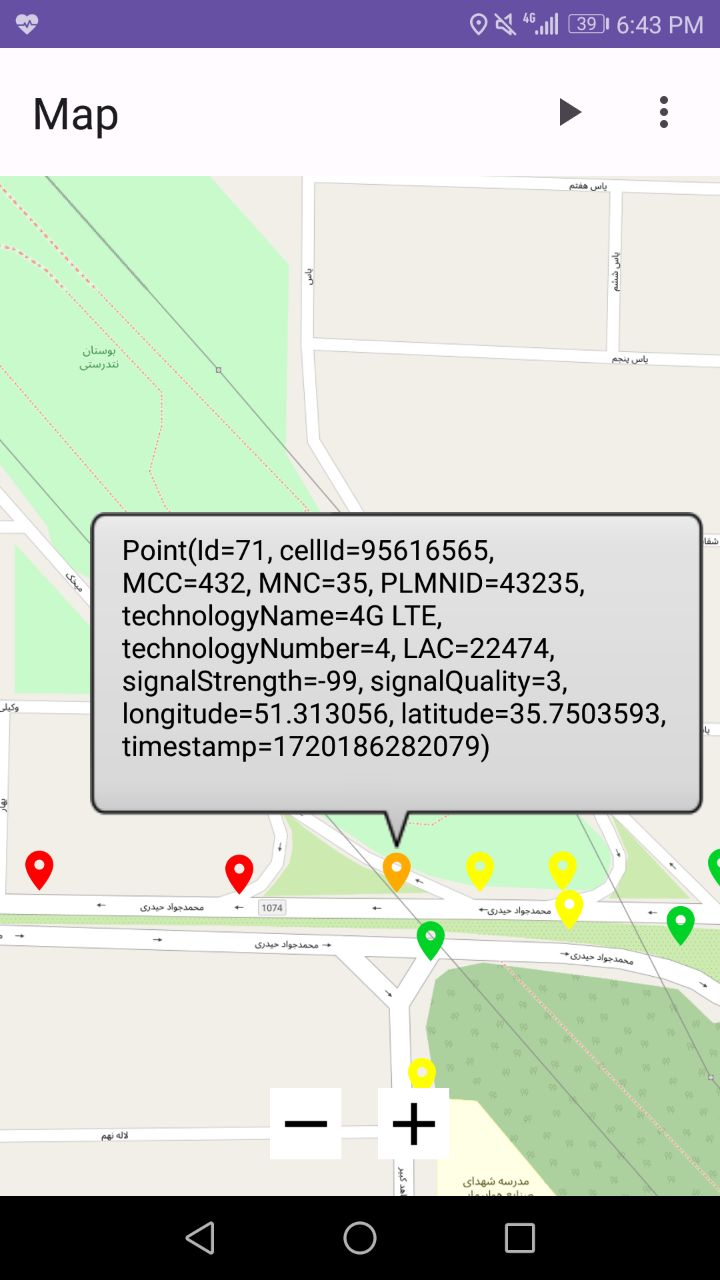
\includegraphics[width=0.4\textwidth]{../images/detail.jpg}
            \caption{اطلاعات مربوط به هر نقطه ثبت شده}
      \end{figure}
\end{center}

\section{صفحه درباره ما}
\begin{center}
      \begin{figure}[H]
            \centering
            
\includegraphics[width=0.4\textwidth]{../images/about_us.png}
            \caption{صفحه درباره ما}
      \end{figure}
\end{center}

\end{document}
